\documentclass[11pt,letterpaper]{article}
\usepackage{apacite}
\usepackage[margin=0.8in]{geometry}
\linespread{1.1}

\usepackage{graphicx,textcomp}
\usepackage{setspace}
\usepackage{fullpage}
\usepackage{color}
\usepackage[reqno]{amsmath}
\usepackage{amsthm}
\usepackage{fancyvrb}
\usepackage{amssymb,enumerate}
\usepackage[all]{xy}
\usepackage{lscape}
\newtheorem{com}{Comment}
\usepackage{float}
\newtheorem{lem} {Lemma}
\newtheorem{prop}{Proposition}
\newtheorem{thm}{Theorem}
\newtheorem{defn}{Definition}
\newtheorem{cor}{Corollary}
\newtheorem{obs}{Observation}
\usepackage[compact]{titlesec}
\usepackage{dcolumn}
\usepackage{tikz}
\usetikzlibrary{arrows}
\usepackage{multirow}
\usepackage{xcolor}
\newcolumntype{.}{D{.}{.}{-1}}
\newcolumntype{d}[1]{D{.}{.}{#1}}
\definecolor{light-gray}{gray}{0.65}
\usepackage{url}

\usepackage{listings}
\usepackage{color}

\definecolor{codegreen}{rgb}{0,0.6,0}
\definecolor{codegray}{rgb}{0.5,0.5,0.5}
\definecolor{codepurple}{rgb}{0.58,0,0.82}
\definecolor{backcolour}{rgb}{0.95,0.95,0.92}

\lstdefinestyle{mystyle}{
	backgroundcolor=\color{backcolour},   
	commentstyle=\color{codegreen},
	keywordstyle=\color{magenta},
	numberstyle=\tiny\color{codegray},
	stringstyle=\color{codepurple},
	basicstyle=\footnotesize,
	breakatwhitespace=false,         
	breaklines=true,                 
	captionpos=b,                    
	keepspaces=true,                 
	numbers=left,                    
	numbersep=5pt,                  
	showspaces=false,                
	showstringspaces=false,
	showtabs=false,                  
	tabsize=2
}
\lstset{style=mystyle}
\newcommand{\Sref}[1]{Section~\ref{#1}}
\newtheorem{hyp}{Hypothesis}


\title{Dublin Bikes Report} 
\date{19/04/2023}
\author{Caitlín Cooney \& Jack Merriman}

\begin{document}
	\noindent \textbf{Dublin Bikes Report - 19/04/2023}\\
	\textbf{Caitlín Cooney \& Jack Merriman}
\paragraph{}
	The two tasks chosen by our research team are:\\
	\textbf{1.} To assess the impact of the pandemic on the city-bike usage;\\
	\textbf{2.} To estimate how the city-bike usage would have been without the pandemic.
\paragraph{Station Selection:}
	To decrease computational times we decided to focus on three bike stations. Before station selection, we used one quarterly dataset to extract all unique stations and their coordinates with R’s \texttt{dplyr} package, on which we performed our selection process in Python.
\paragraph{}
	Rather than choose our three stations arbitrarily, we used the \textit{k-means} clustering algorithm to divide Dublin’s stations with 40 stands into $k = 3$ clusters based on latitude and longitude. This ensures an unbiased selection of $3$ stations representing various parts of Dublin’s geography without any being on the periphery of the network (Fig. 1).\\
\begin{figure}[h]
	\centering
	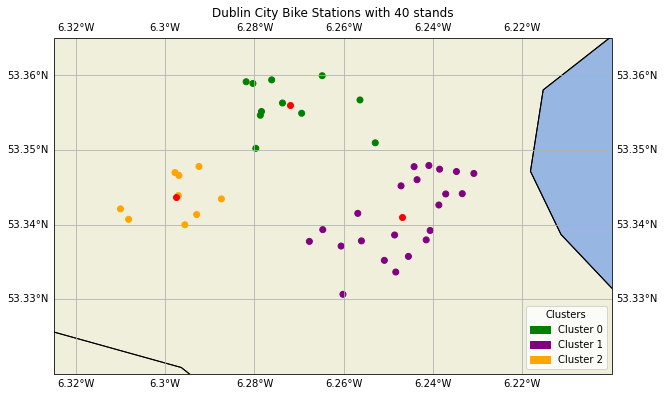
\includegraphics[width=10cm]{kmeans.png}
\end{figure}
\paragraph{}
	Once our clusters were calculated, we found the minimum value of Euclidean distance between the centroid and stations of each cluster. The stations selected through this process were: \textbf{Phibsborough Road, Merrion Square South, Royal Hospital}
\paragraph{Data Pre-processing:}
	Once our stations were selected, we used R’s \texttt{dplyr} to combine quarterly data into a working dataset. When importing the quarterly data into R we filtered observations corresponding to our stations, and then selected relevant variable columns: Station name; time (independent variable); bike stands and available bikes/bike stands (for calculating our dependent variable); and status (in case normalisation was necessary). They were compiled into a single table which was exported for use in Python.
\paragraph{}
	In Python we create a new variable for bike usage, which at timestamp $i$ is calculated as:\\
	$Y\textsubscript{i} = \frac{X1\textsubscript{i}}{X2\textsubscript{i}}$
\paragraph{}
	Where $Y$ is bike usage, $X1$ is available bike stands and $X2$ is total bike stands. We then calculated the average usage across each week in the dataset in order to filter out variation based on day of the week and time of day. This has the added benefit of increasing processing times and making visualisations more legible. The average weekly usage is our final dependent variable and is visualised across the dataset in Figure 2.
\begin{figure}[h]
	\centering
	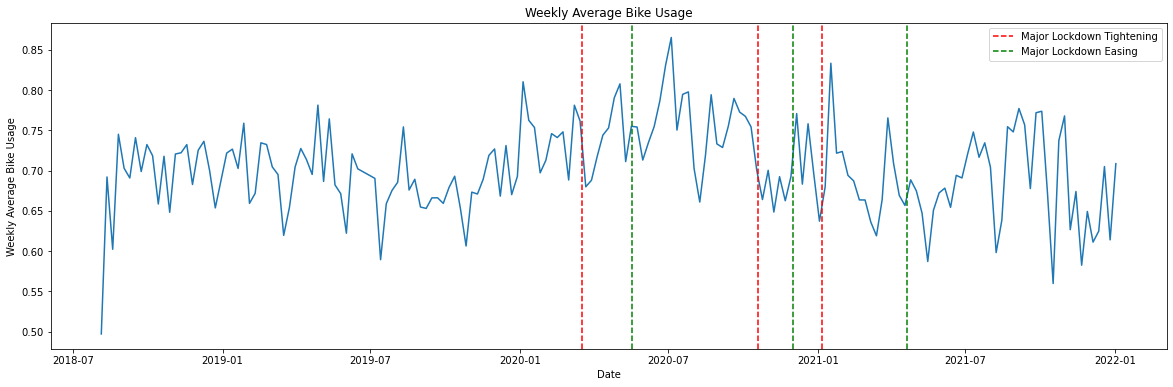
\includegraphics[width=\textwidth]{timeseries.png}
\end{figure}
	
\paragraph{Task 1: Pandemic Impact}
	To assess the impact of the pandemic, we run a linear regression analysis on bike usage prior to the pandemic, and comparing this with the same model run on data after lockdown restrictions were brought in. First we divided our data into pre-pandemic and post-pandemic periods, with a cutoff of March 15th, 2020 (as it was this week that restrictions were brought in). We then dropped any missing values, as there were 18 days of missing data in June 2019. Finally we transformed our time variable by numbering each week (1-179). This made our sole feature (time) compatible with our model code.
\paragraph{}
	With the data prepared, we used \texttt{sklearn}’s linear regression module to regress weekly average bike usage on week number to show the trend for each period (Fig 3). The equations for each line are as follows:\\
	\textbf{Pre-pandemic:} \hspace{4.6cm} \textbf{Post-pandemic:}\\
	$Y = 0.00026794X + 0.68513153$ \hspace{2.2cm} $Y = -0.00099054X + 0.8387338$
\begin{figure}[h]
	\centering
	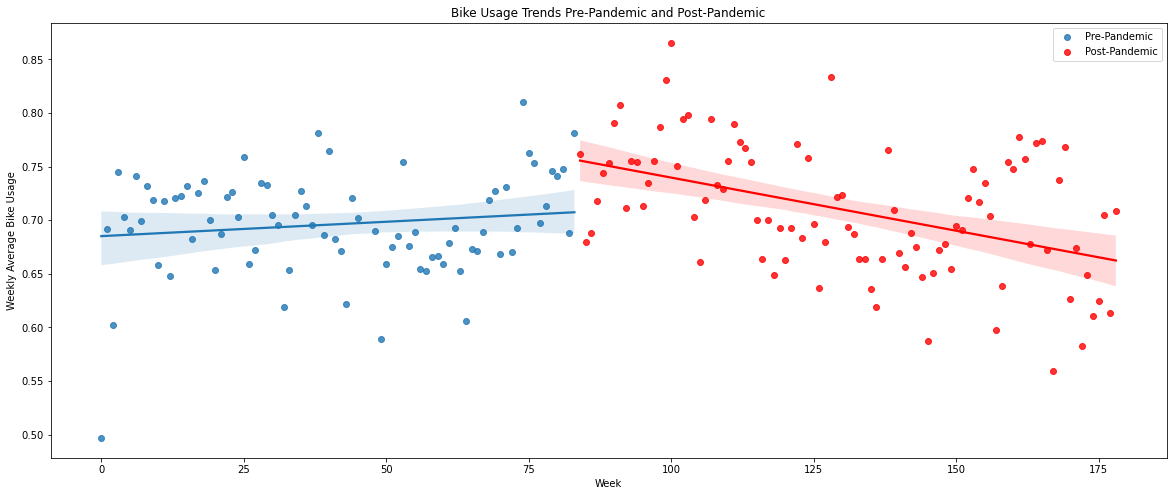
\includegraphics[width=\textwidth]{comparison.png}
\end{figure}
\newpage
\paragraph{}
	Most noticeably, there is a sharp increase in the constant value of the post pandemic line. A mild positive trend gives way to stronger decline in average bike usage after the initial spike. A possible explanation for the sharp increase following the onset of the pandemic is the significant drop in motor traffic on Irish roads due to mobility restrictions \cite{traffic}, as quieter roads decrease the perceived risk of cyclists and likelihood of uptake \cite{risk}. The negative trend suggests a reversion to the mean as the effects of the initial shock of the pandemic wane.\\
\paragraph{Task 2: Counterfactual Estimation}
	To estimate city-bike usage in a counterfactual situation with no pandemic, we used the same modelling method as the pre-pandemic data in Task 1, but this time using an 80:20 train/test split for cross-validation to ensure predictions would be useful. We calculated the mean squared error of our linear model for the training set, the testing set, and a static null array of the mean pre-pandemic average weekly bike usage.
\paragraph{}
	\textbf{train MSE = 0.001938, test MSE = 0.003058, null MSE = 0.003093}
\paragraph{}
	This shows that while our model is well validated, that the trend is not very different from a static line based on the mean of the data, showing that there was no significant positive trend, rather a stagnation. We then used our pre-pandemic model to predict values for post-pandemic weeks, showing counterfactual estimates (Fig. 4).
\begin{figure}[h]
	\centering
	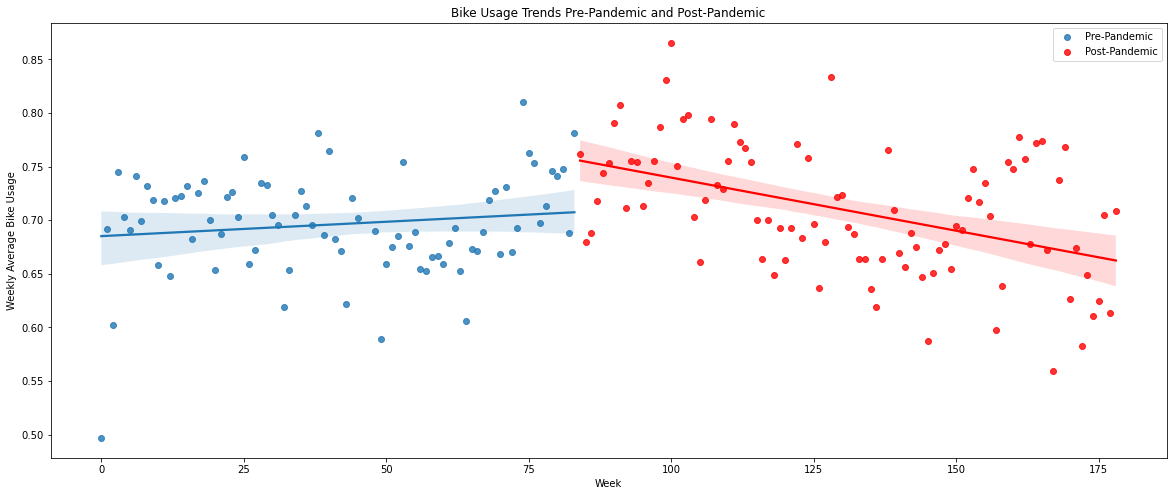
\includegraphics[width=\textwidth]{comparison.png}
\end{figure}
\paragraph{}
	The final difference in predicted values (X=179) is just over 0.01, showing that although the pandemic had a large initial impact on bike usage, its impact does not significantly differ from a counterfactual non-pandemic prediction in the long term.
\newpage

\bibliographystyle{apacite}
\bibliography{bike}

\noindent \textbf{Appendix 1: Division of work}\\

Both members of the group were present together for the entirety of the work on this project, and as such every item of work was a joint effort. Although we both prioritised different items according to our strengths, both members contributed ideas and troubleshooting for the other’s priorities. \\

Data wrangling in R, pre-processing in Python, data visualisation and counterfactual predictions for task 2 were prioritised by Jack.\\

Coding of clustering algorithms, coding of linear regression models, and model cross-validation/evaluation were prioritised by Caitlín.\\

\noindent \textbf{Appendix 2: GitHub}\\

R scripts for data-wrangling and Jupyter notebook files for completion of the tasks, the .csv data files as well as the \LaTeX\hspace{0.05cm} code and figures of this report can be found in this project’s GitHub repository here: https://github.com/jackmerriman/MLProject


\end{document}
